\documentclass{stdlocal}
\begin{document}
\section{Implementation} % (fold)
\label{sec:implementation}
  In the section \ref{sec:pseudorandom_number_generators}, we have already discussed the mathematical foundations of PRNGs, as well as some examples, like the MT19937.
  In this section, we will first implement a scalar variant of the chosen generators to better understand their structure and design.
  Moreover, they serve as a testing facility to make sure the output of the vectorized PRNGs is correct.
  After explaining the critical points in the implementation, we will show how to vectorize the given generators.
  For this, it is helpful to first discuss which technique to use for the vectorization.
  Afterwards a theoretical analysis of the used vector intrinsics concerning their latency and throughput will follow to pinpoint bottlenecks of the implementation possibly resulting in future work.

  \subsection{MT19937} % (fold)
  \label{sub:mersenne_twister}
    The MT19937 is the de facto standard of applications using random numbers to compute their results.
    In the original paper, \citeauthor{matsumoto1998} have given a standard implementation in the C programming language.
    % This implementation is easily adjustable to work in C++.
    To map the C-style functional programming to modern C++ paradigms, we introduce a functor that stores the complete state of the Mersenne twister.
    The functional operator is then used to represent the application of the transition and generator function to receive a new random number.
    The introduction of the functor grants us the complete power of the C++ template, type, and class system while preserving an easy-to-use interface.

    \inputCodeBlock[title = Scalar MT19937 Structure]{code/mt19937/sisd/struct.hpp}
    In \textcite{kneusel2018}, a special seeding routine was used, such that the actual initialization process only needs one truly random number.
    In the STL of the C++ programming language the MT19937 is already implemented.
    The corresponding class is called \code{std::mt19937} and offers a constructor with only one integral number of 32-bit length as seeding value.
    This constructor uses the initialization routine described by \textcite{kneusel2018}.
    We want to make sure, that our implementation gives exactly the same output as the standard variant while keeping the advantages of our own API.
    As a consequence, we have to introduce another structure \code{default_seeder} which can be interpreted as a PRNG and should also be able to serve as a default seeder for the MT19937.
    The implementation of \code{default_seeder} is constructed in the same way as it was done for the MT19937 itself.
    First, we introduce a functor with the appropriate state while using the function operator as advancing routine.
    The initialization from \textcite{kneusel2018} was slightly changed to adapt to the new functor definitions.
    By designing a fast-forward constructor, it is possible to seed our own MT19937 with any other RNG including the default seeder.

    \inputCodeBlock[title = Scalar MT19937 Seeding]{code/mt19937/sisd/seeding.hpp}
    The types and parameters of the MT19937 will be defined as compile-time constants inside the functor to make sure the code stays maintainable by not inserting magic numbers in the implementation of the advancing routine.
    To guarantee that there is no runtime overhead, we define those variables as \code{static constexpr}.
    Please note that we could use a class template to parameterize such member types and constants as it is done in the STL.
    However, in consideration of the fact that we only want to vectorize the MT19937 of the Mersenne Twister family, it is completely sufficient to use non-template types and constants.
    The code is given in the appendix in listing \ref{code:mt19937-scalar-constants}.

    Advancing the state of the MT19937 by asking for a random number is a more complicated algorithm.
    The recurrence of the Mersenne twister is linear and gives us an equation on how to get to the next element based on the 624 current elements.
    According to the mathematics, after the computation we would have to move every element of the state one step further, as can be seen in figure \ref{fig:mersenne-twister-transition-generation}.
    But accessing each element in the state vector for every random number would greatly reduce the performance due to cache misses and the time to move every element.
    Instead, \citeauthor{matsumoto1998} cache the index of the current element in the state and are precomputing 624 steps of the transition function.
    This guarantees that newly generated elements do not have to be moved to the end of the state but instead can reside at their current positions.
    Because we are transforming every state element by applying the transition function 624 times, the precomputation step has to loop over all elements.
    To make sure the transformation is only accessing elements that lie inside the state, the loop has to be split into three distinct parts.
    The transition of a single element depends on two other elements in the state.
    Every dependency introduces a split because it could lie outside the state by shifting forward.
    In figure \ref{fig:mt-loop-scheme}, this process is shown schematically.

    \begin{figure}
      \center
      \begin{subfigure}[b]{0.26\textwidth}
        \center
        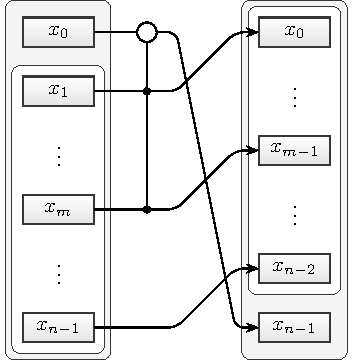
\includegraphics[width=0.95\textwidth]{figures/mt19937_transition_short.pdf}
      \end{subfigure}
      \begin{subfigure}[b]{0.71\textwidth}
        \center
        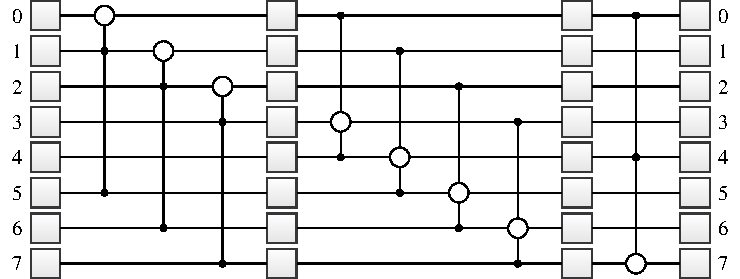
\includegraphics[width=0.95\textwidth]{figures/mt19937_loop_scheme.pdf}
      \end{subfigure}
      \caption[Mersenne Twister Loop Scheme]{
        Implementation of the Mersenne twister by precomputing its transition through a loop over the elements in the state.
        The left image shows a shorthand notation for a single call to the transition function.
        The right image visualizes the loop over all elements by using the simpler notation for a simplified version of the Mersenne Twister with a state size of eight and a shift size of five.
      }
      \label{fig:mt-loop-scheme}
    \end{figure}

    While the cached index is small enough, advancing the state only results in incrementing the index and returning the state value at this position by applying the generator function.
    Only if the index reaches the end, the complete state vector will be regenerated with respect to the recursive relation.
    In our code, the regeneration of the state vector uses a lambda expression to reduce code duplication and improve code transparency.
    The lambda expression keeps the code local in contrast to helper or member functions.
    Hence, the compiler will probably inline all calls to the lambda expression optimizing the scalar code in the best possible way.

    \inputCodeBlock[title = Scalar MT19937 Advancing]{code/mt19937/sisd/advance.hpp}
    The design of our Mersenne Twister ensures that the output will be the same as the output of the MT19937 from the STL of the C++ programming language.
    Additionally, the interface provides a more general seeding variant which improves statistical performance for seeding generators other than the default seeder.
    The new initialization facility is easier to use and gives a better {}insight into the used seeding values to the reader of the code.
    The function to advance the state is easier to understand, maintainable and generalizable.
    Last but not least, as we will show, our MT19937 implementation is able to provide a better performance in an actual application.

    Because the state of the MT19937 is very large in comparison to the size of the SSE and AVX vector registers, we rely on a typical vectorization technique described by \textcite{fog2015} that does not need to initialize multiple instances of the same generator.
    The scalar implementation offers a large degree of data independence.
    After the regeneration of the complete state vector, the generator function has to be applied on each individual element to provide random numbers.
    This problem describes the perfect use case for SIMD intrinsics.
    In the AVX case, we can read eight 32-bit values at the same time by the usage of a vector register and apply the generator function on each element in parallel by using the respective intrinsics.
    In the SSE case, we would only read four elements.
    The number of elements in the state vector is divisible by eight and four without remainder.
    Hence, we do not have to take care of the boundaries of the state vector.

    \inputCodeBlock[title = AVX MT19937 Structure]{code/mt19937/simd256/struct.hpp}
    The structure of the vectorized version does not introduce major changes to the underlying design.
    We make sure that the state vector will be at least 32-byte aligned to exploit faster loading and storing operations while advancing the state.
    To further optimize the structure, we could force 64-byte alignment to provide improved caching possibilities by letting the state start at a cache line boundary.

    The moment every package of eight or four elements in the state vector is read, the regeneration has to be triggered.
    The computation of the new state vector exhibits some data dependencies we have to take care of.
    In the scalar variant of the regeneration process the loop of all elements was split into three parts --- one for the first 227 elements, one for the following 396 elements and one for the last element.
    The splitting followed from the dependencies given by the recurrence defining the Mersenne twister algorithm.
    All elements in the first loop have to access the elements at the same position, one position ahead and 397 steps ahead.
    Reaching the 227th~element will then forbid us to go 397 steps further, because the position would not lie inside the state vector.
    But the requested element has already been produced at position zero.
    Therefore all elements in the second loop need to access the elements at the same position, one position ahead and 227 steps backwards.
    For the last element the successive element would again lie outside the state vector.
    Hence, the last elements uses the elements at the last position and positions zero and 396.

    \begin{figure}
      \center
      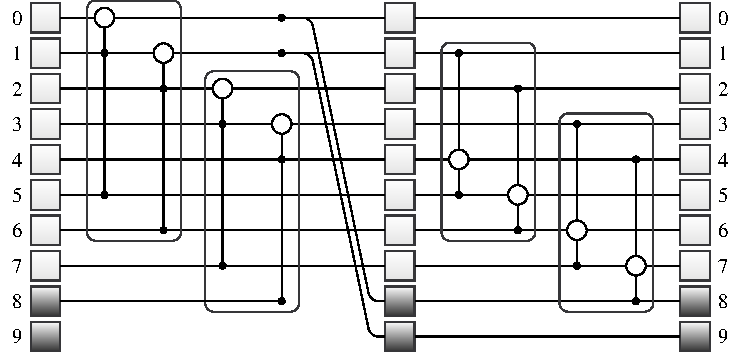
\includegraphics[width=0.95\textwidth]{figures/mt19937_vector_loop_scheme.pdf}
      \caption[Mersenne Twister Vector Loop Scheme]{
        Vectorization of the loop of Mersenne twister implementation by adding a buffer (gray) with the size of an SIMD vector at the end of the state.
        Here, the same simplified version as in figure \ref{fig:mt-loop-scheme} is used.
        It is assumed SIMD vectors are able to contain two elements of the state at once.
        Vectorizable operations are shown in boxes.
        By copying the first vector containing the new state elements into the buffer, no SIMD vector will overlap the first and the second loop.
      }
      \label{fig:mt-vector-loop-scheme}
    \end{figure}

    Thus, all newly generated elements in the first loop are independent of each other and can therefore be vectorized.
    This is also true for the second loop after the first loop has been executed.
    The problem lies in the fact that the number 397, as well as 227, is not divisible by eight or four without remainder.
    This leads to the appearance of a boundary vector term for the last element at the end of the state vector and one between the first and the second loop which needs to access successive and previous elements at the same time.
    Handling these boundary terms explicitly through vector intrinsics will result in complex loading, storing and blend operations.
    We have chosen another path by slightly changing the layout of the underlying data structure.
    Instead of saving only 624 elements for the state vector, we append values at the end of the state vector to get a buffer that should reduce complexity.
    The number of values we append is given by the amount of elements that fit into a vector register.
    After the generation of the first vector unit in the first loop, we will copy these values to the end into the buffer.
    In this case, the last value in the state vector will no longer be a boundary term because it can access the consecutive elements through the buffer.
    The boundary term between the first and the second loop can now be completely handled by the vectorized first loop.
    The new vectorization scheme of the complete loop is shown in figure \ref{fig:mt-vector-loop-scheme}.
    This method makes the code implementation easier by making the state bigger.
    But the number of elements we put into the buffer is small in comparison to the MT19937 state size and therefore an acceptable price to pay.

    % \inputCodeBlock[title = AVX MT19937 Advancing]{code/mt19937/simd256/advance.hpp}

    \inputCodeBlock[title = AVX MT19937 Advancing]{code/mt19937/simd256/advance.hpp}
    Because the state vector is aligned, we can exploit this by using aligned load operations for elements that will be used without a shift.
    For all other elements, we still have to use unaligned load operations.
    All parts in the vectorized advancing routine are then directly translated into their corresponding vector intrinsics.

    Except \code{_mm256_cmpgt_epi32}, all AVX intrinsics which are used in the code exhibit a latency of $1$ on the typical microarchitectures.
    \code{_mm256_cmpgt_epi32} has a latency of $3$ and a throughput of $1$ and therefore represents some kind of bottleneck that cannot be avoided.
    The throughput for loading and storing vector values is $0.25$.
    Hence, the loading of the three dependent values in the transition function should run in parallel.
    To even tweak the code further, we could always use two AVX vector registers at the same time by interleaving their operations.
    This would exploit the lower throughput of other intrinsics.
    In this case, only the shift operations in the generation function, like \code{_mm256_slli_epi32}, would bound the overall performance due to their throughput of $1$.
    \autocite{intel-intrinsics-guide,fog2019d}

    In listing \ref{code:mt19937-avx-advance-asm}, the assembly code of the vectorized advancing routine is shown.
    We have compiled the source code through the use of \citetitle{compiler-explorer} with the highest degree of optimization enabled \autocite{compiler-explorer}.
    It can be seen that the AVX intrinsics that were used for the implementation could directly be translated to their according assembler instructions.
    Besides, the optimization of the compiler is still active and helps to further exploit latencies and throughputs automatically.
    Hence, the use of SIMD intrinsics in C++ code can be seen as superior in comparison to writing inline assembly code.
  % subsection mersenne_twister (end)

  \subsection{Xoroshiro128+} % (fold)
  \label{sub:xoroshiro}
    The scalar implementation of the Xoroshiro128+ follows the same rules as the scalar implementation of the MT19937.
    \citeauthor{vigna-xoroshiro} provides the C code for the generator on his website \autocite{vigna-xoroshiro}.
    We again use a functor which saves the state and advances it by calling the function operator.
    Compile-time constants will again be declared as \code{static constexpr} to reduce the runtime overhead.
    In comparison to the MT19937, the state of the Xoroshiro128+ can be easily described by two 64-bit unsigned integer values.
    Hence, we only show the data structure in the appendix in code snippet \ref{code:xoroshiro-scalar-struct}.
    For the advancing routine, the generator needs a utility which is rotating the bits of a 64-bit unsigned integer.
    % \inputCodeBlock[title = Scalar Xoroshiro128+ Structure]{code/xoroshiro128plus/sisd/struct.hpp}
    Furthermore, the Xoroshiro128+ offers a jump-ahead feature for discarding $2^{64}$ or $2^{96}$ elements of the output.
    In listing \ref{code:xoroshiro-scalar-jump}, we are only providing the implementation of the smaller jump.
    Both jumping routines differ only in their masking numbers.
    % The testing of the jump functions seems to be problematic because we have no possibility of generating $2^{64}$ random numbers in a short time to check if state of the PRNG is the same after a call to the jump function.
    % One workaround is to check each jump against each other by executing $2^{32}$ small jumps

    \inputCodeBlock[title = Scalar Xoroshiro128+ Advancing]{code/xoroshiro128plus/sisd/advance.hpp}
    Due to the small state size of the Xoroshiro128+, the vectorization has to use multiple instances of the same generator to exploit the full capabilities of the SIMD intrinsics.
    \citeauthor{vigna-xoroshiro} only gives one parameter set for the PRNG.
    As a consequence, we have to use different seeds for all instances possibly causing overlapping subsequences or the jump-ahead feature to make sure the instances do not overlap for at least $2^{64}$ or $2^{96}$ values.
    For the AVX implementation, we will use four instances of the Xoroshiro128+.
    The underlying structure therefore does not really change and uses the SIMD types instead of the 64-bit unsigned integer types.
    The layout of the data structure for the AVX version can be seen in figure \ref{fig:xoroshiro-vector-layout}.

    \begin{figure}
      \center
      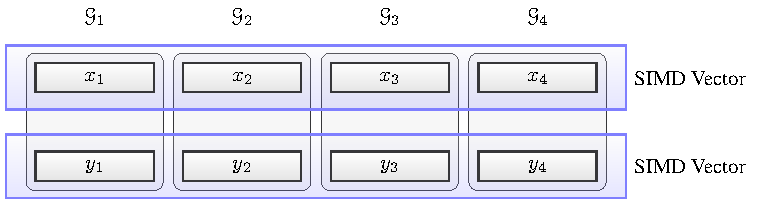
\includegraphics[width=0.95\textwidth]{figures/xrsr128p_vector_layout.pdf}
      \caption[Xoroshiro128+ Vector Layout]{%
        Memory layout concerning SIMD vectors of four instances of the Xoroshiro128+.
        SIMD vectors are shown as blue box.
      }
      \label{fig:xoroshiro-vector-layout}
    \end{figure}

    % \inputCodeBlock[title = AVX Xoroshiro128+ Structure]{code/xoroshiro128plus/simd256/struct.hpp}
    With this approach, every instance of the generator is completely independent of the other instances.
    This is again perfect for the application of SIMD intrinsics.
    The AVX implementation of the advancing routine is therefore straightforward because we are able to interchange every scalar instruction with its corresponding vector intrinsic.

    \inputCodeBlock[title = AVX Xoroshiro128+ Advancing]{code/xoroshiro128plus/simd256/advance.hpp}
    Due to the latencies and throughputs of the AVX intrinsics used in this implementation, the advancing routine does not introduce a major bottleneck in the generation of random numbers.
    But to exploit the throughput of every operation, we would need to use multiple independent SIMD vector registers at once.
    This would increase the number of SIMD registers in the return type of the function as well.

    The jump function, given in listing \ref{code:xoroshiro-avx-jump}, uses a branch in the inner loop to decide which code path to execute.
    We do not want this branch to slow down the code by switching to scalar-execution mode.
    Hence, we will map the branch to vector intrinsics by executing the inner computation in every case and masking the result based on the vectorized evaluation of the branch condition.
    Seeding the AVX version of the Xoroshiro128+ with the usage of the vectorized jump routine can then be done by first initializing the four instances with the same random seed.
    Afterwards, three vectorized jumps have to be executed.
    For every step, we have to use masking operations to make sure the jumping is only executed for the instances in the AVX register that have to advance further.
    So after the computation of the first jump, the first instance has to be masked.
    For the second step, only the third and the fourth instance should change and therefore the first and the second instance are masked.
    The third jump then only has to be done for the fourth instance.

    In the code \ref{code:xoroshiro-avx-advance-asm}, \ref{code:xoroshiro-avx-advance2-asm}, and \ref{code:xoroshiro-avx-advance4-asm}, we provide the assembly code generated by \citetitle{compiler-explorer} for calling the advancing routine once, twice, and four times, respectively \autocite{compiler-explorer}.
    As before, all AVX intrinsics were correctly translated into their respective assembler instructions.
    Looking at the listings \ref{code:xoroshiro-avx-advance2-asm} and \ref{code:xoroshiro-avx-advance4-asm}, we even see that the compiler completely inlined multiple calls to the advancing routine automatically.
    In contrast to the MT19937, the AVX implementation of the Xoroshiro128+ enables us to keep using the vector registers without cache or memory communication while generating new random numbers.
    This property will provide a higher performance as we will see in the evaluation process.

  % subsection xoroshiro (end)

  \subsection{MSWS} % (fold)
  \label{sub:middle_square_weyl_generator}
    The MSWS is a simple, modern, and non-linear PRNG that uses a state which is based on 64-bit unsigned integer values but is returning only a 32-bit unsigned integer.
    The scalar implementation will again use the same approach as the MT19937 and the Xoroshiro128+ as it is given as a C implementation in \textcite{widynski2019}.
    The seeding routine for the MSWS is more complicated and requires a more sophisticated algorithm.

    \inputCodeBlock[title = Scalar MSWS]{code/msws/sisd/struct.hpp}
    The MSWS does not provide different parameters or a jump-ahead feature.
    Its small state size requires us to use multiple instances of independent generators to exploit the size of the vector registers.
    Thus, all instances have to be initialized with different seeds possibly generating overlapping subsequences.
    But because its output is only given by a 32-bit value, we have to generate eight random numbers at once.
    We can decide to call four instances of the same generator twice or instead use eight instances.
    While benchmarking the generators, the variant for calling each instance twice reduced the actual throughput of the vectorized PRNG and was therefore discarded from the implementation and measurement.
    In our vectorized implementation, we use eight instances of the MSWS.
    A visualization of the data structure layout is given in figure \ref{fig:msws-vector-layout}.

    \begin{figure}
      \center
      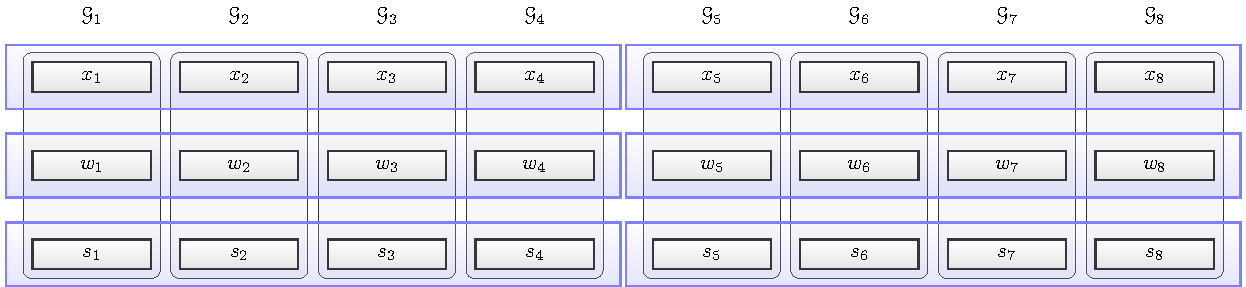
\includegraphics[width=0.95\textwidth]{figures/msws_vector_layout.pdf}
      \caption[MSWS Vector Layout]{%
        Memory layout concerning SIMD vectors of eight instances of the MSWS.
        SIMD vectors are shown as blue box.
      }
      \label{fig:msws-vector-layout}
    \end{figure}

    % \inputCodeBlock[title = AVX MSWS Structure]{code/msws/simd256/struct.hpp}
    Advancing the state of the vectorized MSWS introduces difficulties because we have to compute the square of the first 64-bit value.
    Neither the AVX nor the SSE instruction set is providing a multiplication or squaring operation for 64-bit unsigned integer numbers.
    Accordingly, we have to implement our own function for squaring the 64-bit values in a vector register based on given intrinsics.
    For this, we will map the 64-bit multiplication to 32-bit multiplications.
    Let $x\in\setInteger_{2^{64}}$ be a 64-bit unsigned integer and let $x_0,x_1\in\setInteger_{2^{32}}$ be its 32-bit representation, such that
    \[
      x = x_1 2^{32} + x_0 \ .
    \]
    We are then able to formulate the squaring of this number in 64-bit arithmetic by using modulo and the binomial formula.
    \begin{align*}
      x^2
      &= x_1^2 2^{64} + 2x_1x_0 2^{32} + x_0^2 \\
      &\equiv 2x_1x_0 2^{32} + x_0^2 \mod 2^{64}
    \end{align*}
    Due the modulo, the product $x_1x_0$ only needs to use a 32-bit multiplication.
    The value $x^2_0$ can be fully expressed by a 64-bit integer type.
    Hence, we have to use a 64-bit multiplication for 32-bit number $x_0$ to deal with the carry bits of the computation $x_0^2$.
    The SSE and AVX instruction sets provide this operation, such that the added complexity of the computation can be used to find an optimal implementation.

    Afterwards, the first part of the vectorization is again straightforward because all the instances are independent so that every statement can directly be interchanged with its corresponding vector intrinsic.
    At the end of the first part, two variables of SIMD type will provide 64-bit values as random numbers.
    The MSWS algorithm forces us to use only the lower 32-bit of the given values resulting in only one vector type with the doubled amount of values as result.
    To do that, both variables have to be convoluted by shuffle or permutation operations.
    Two variants are shown in figure \ref{fig:msws-vector-merge-scheme}.
    % The squaring function and the permutation operations at the end will probably exhibit a high latency and therefore reduce the speed-up of the vectorization.

    \begin{figure}
      \center
      \begin{subfigure}[b]{\textwidth}
        \center
        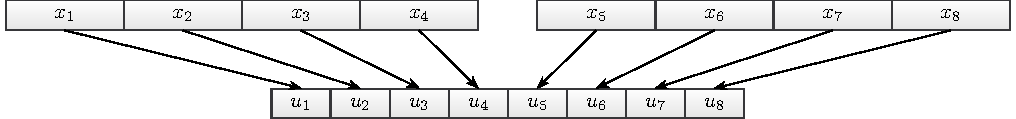
\includegraphics[width=0.95\textwidth]{figures/msws_merge.pdf}
        \caption{Sequential.}
      \end{subfigure}

      \begin{subfigure}[b]{\textwidth}
        \center
        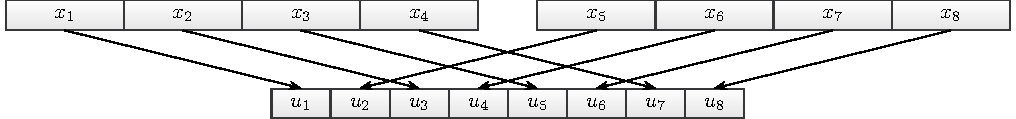
\includegraphics[width=0.95\textwidth]{figures/msws_merge2.pdf}
        \caption{Interleaved.}
      \end{subfigure}
      \caption[MSWS Vector Merge Scheme]{%
        Two variants of merging the two output vectors of the vectorized MSWS containing 64-bit integers into one SIMD vector containing 32-bit integers by means of AVX vector registers.
      }
      \label{fig:msws-vector-merge-scheme}
    \end{figure}

    \inputCodeBlock[title = AVX MSWS Advancing]{code/msws/simd256/advance.hpp}
    In the AVX implementation, we use \code{_mm256_mul_epu32} and \code{_mm256_mullo_epi32} to compute the square of the first element in the state.
    They exhibit a latency of $5$ and $10$ and a throughput of $0.5$ and $1$ on the typical microarchitectures, respectively.
    Thus, in comparison to the other intrinsics, they tremendously reduce the performance of the advancing routine.
    To exploit their throughput, we would have to run ten of these instructions for independent AVX vectors consecutively.
    One 256-bit SIMD vector contains four 64-bit MSWS generators.
    Therefore at least 40 instances of the PRNG have to be called in parallel to remove the latency bottleneck of the multiplication operations.
    Due to the risk of lowering the statistical quality, we have only used eight generators in parallel.
    \autocite{intel-intrinsics-guide,fog2019d}
  % subsection middle_square_weyl_generator (end)

  \subsection{Uniform Distribution Functions for Reals} % (fold)
  \label{sub:uniform_real_distribution}
    The uniformly distributed transformation of random 32- and 64-bit integers to single- and double-precision floating-point values is described in \textcite{vigna-xoroshiro} and \textcite{kneusel2018}.
    Here, the IEEE 754 floating-point standard is used to ensure that bit manipulations will result in the same number on every machine supporting this standard.
    Because we only want to deal with normalized numbers, a value in the interval $[1,2)$ should be generated firstly.
    Such a value is positive and therefore the sign bit of the floating-point value is set to $0$.
    The actual number representing the exponent of the floating-point encoding should be zero.
    Due to the offset applied to the exponent value, the content of the exponent has to be equal to the offset.
    Then the fraction can be filled with random bits to construct a uniformly distributed floating-point value in the interval $[1,2)$.
    Low-order bits of a pseudorandom integer tend to provide weak randomness properties.
    Hence, a shift is used to fill the fraction with the most significant bits of the random integer.
    In figure \ref{fig:real-uniform-implementation-scheme}, this can be seen for a 32-bit integer and a single-precision floating-point value.
    After this computation, the remaining part has to subtract $1$ from the floating-point value to guarantee the uniform distribution in the unit interval $[0,1)$.
    The scalar implementation is given in the following code snippet.

    \begin{figure}[h]
      \center
      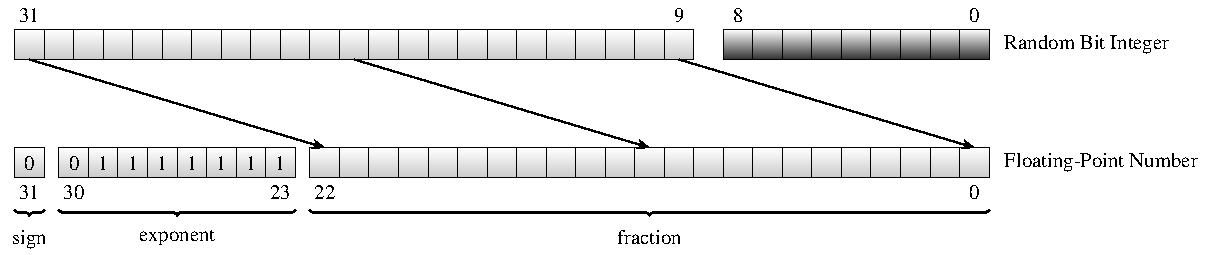
\includegraphics[width=0.95\textwidth]{figures/uniform_implementation_scheme.pdf}
      \caption[Real Uniform Distribution Function Implementation Scheme]{%
        Generating a uniformly distributed floating-point number by shifting bits of a given random integer of the same size.
        According to the IEEE 754 floating-point standard, sign and exponent bits have to be set, such that the number will be in the interval $[1,2)$.
      }
      \label{fig:real-uniform-implementation-scheme}
    \end{figure}

    \inputCodeBlock[title = Scalar Uniform Function]{code/uniform/sisd/uint32.hpp}
    \newpage
    \noindent
    The vectorization of the uniform routine is straightforward.
    Every operation can be replaced by its respective intrinsic.
    Analyzing the function, \code{_mm256_sub_ps} and \code{_mm256_sub_pd} exhibit the highest latency with a value ranging from $3$ to $4$ on typical microarchitectures \autocite{intel-intrinsics-guide,fog2019d}.
    On the other hand, their throughput ranges from $0.5$ to $1$.
    So to further improve the performance of the uniform function, multiple independent values should be computed resulting in better exploitation of the processor pipeline.

    \inputCodeBlock[title = AVX Uniform Function]{code/uniform/simd256/__m256i.hpp}
    % \inputCodeBlock[title = AVX Uniform Function with Bounds]{code/uniform/simd256/bounds.hpp}

  % subsection uniform_real_distribution (end)

  % \subsection{Uniform Distribution Functions for Integers} % (fold)
  % \label{sub:uniform_distribution_functions_for_integers}

  % % subsection uniform_distribution_functions_for_integers (end)
% section implementation (end)
\end{document}